\section{Methods}\label{sec:methods}


\subsection{Experimental Setup}\label{sec:experiment}

The TCE  dynamic sorption process of different building materials were determined by use of a method schematically shown in Figure \ref{fig:js_sx_setup}.
This method involved a selected material contained in an adsorption column through which TCE-containing gas was passed, and subsequent thermal desorption and measurement of the total amount of adsorption.
During the adsorption part of the process, stainless steel tubes were packed with building materials held in place by glass wool.
The amount of building material normally held in the tube was around 1 g. % TODO: (I forget which materials we used in this manuscript. drywall=2 g, leather=2 g).
It was determined that neither the glass wool nor the stainless steel tube would retain significant amounts of TCE.
The sample-containing tubes were first exposed desired low concentrations of TCE in nitrogen, which were then allowed to interact with the flow for varying periods of time.
The typical flow rate of the nitrogen was 60 ml/min and the concentrations of TCE was around 1.1 ppbv.
All of these adsorption experiments were conducted at room temperature.
After a given time of exposure to the TCE-containing flow, that flow was stopped, and the sample tube was attached to a sorbent tube placed downstream of the sample tube.
The sample tube was arranged such that the direction of the nitrogen flow in the subsequent desorption process was opposite that of the TCE-containing nitrogen flow during the adsorption process.
During the thermal desorption step, the sample containing tube was covered by a heating mantle which permitted its heating at 100 C. % TODO: Add degree symbols
This allowed fully desorbing the TCE which had been held on the sample into a pure nitrogen flow, which carried it to the room temperature downstream sorbent tube, where it was again fully adsorbed.
These tubes fully capture all of the TCE desorbed, from the samples, and the amount of TCE was analyzed by Gas Chromatography (GC) with an  Electron Capture Detector(ECD).

\begin{figure}
  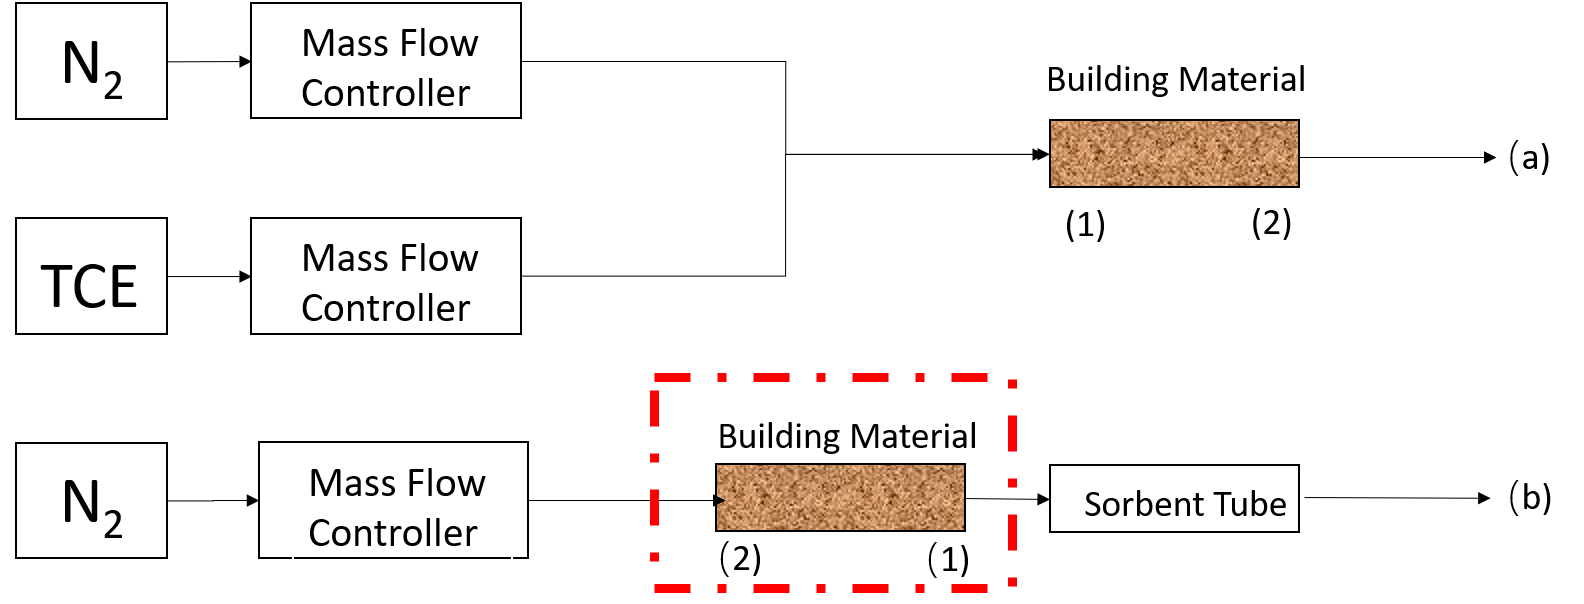
\includegraphics[width=\textwidth]{JS_SX_experiment_setup.png}
  \caption{Schematic of experimental setup.} % TODO: Shuai: Writer better description
  \label{fig:js_sx_setup}
\end{figure}

\subsection{Numerical Model}\label{sec:model}

To investigate the role of sorption in VI, we consider a simple VI scenario.
Here we consider a house with a 10 by 10 m footprint, with the foundation bottom located 1 m below ground surface (bgs).
The sole contaminant source is an uniformly TCE contaminated groundwater located 4 bgs, and the soil surrounding the house is assumed to homogenous and of a singular type.
All contaminant vapors are assumed to enter the house through breaches in the foundation, modeled as a 1 cm wide crack that runs along the perimeter of the house.
Finally we assume that sorption processes can occur both in the soil matrix and in the indoor environment (on various indoor materials).\par

Modeling this scenario requires us to simulate a couple of physics, many of which depend and interact with each other.
The governing equations and the physics they govern are:
\begin{enumerate}
  \item van Genuchten retention model - soil moisture.
  \item Darcy's Law - air flow in the porous media.
  \item Transport equation - contaminant transport in porous media.
  \item Continuously stirred tank reactor (CSTR) - contaminant concentration in the indoor environment.
\end{enumerate}
These physics are implemented in COMSOL Multiphysics, a commercial finite-element method package, which is used to solve our model.
It is important to note that the indoor environment is implicitly modeled, but instead only given by the CSTR equation; the soil domain is explicitly modeled.\par

\subsubsection{Vadose Zone Moisture Content}

Since the contaminant transport occurs through three-phased the vadose zone, it is important that we correctly account for soil moisture content and its effect on advective and diffusive transport.
In this modeled scenario, we assume that the soil moisture is at steady-state and does not change, and thus the soil moisture content is given by the retention model developed by van Genuchten.\par

The van Genuchten retention model gives the soil water saturation as a function of elevation above groundwater.
In turn this gives the water and gas filled porosities, and the relative permeability of the soil matrix.
\begin{align}
  % saturation
  \mathrm{Se} &=
    \begin{cases}\label{eq:van_genuchten_saturation}
      \frac{1}{(1 + \alpha z^n)^m} & z < 0 \\
    1 & z \geq 0
    \end{cases} \\
  % soil moisture
  \theta_w &=
    \begin{cases}\label{eq:van_genuchten_soil_moisture}
      \theta_r + \mathrm{Se}(\theta_s - \theta_r) & z < 0 \\
      \theta_s & z \geq 0
    \end{cases} \\
  % relative permeability
  k_r &=
    \begin{cases}\label{eq:van_genuchten_relative_permeability}
      \mathrm{Se}^l \big[ 1 - \big( 1 - \mathrm{Se}^\frac{1}{m} \big) \big]^2 & z < 0 \\
      0 & z \geq 0
    \end{cases}
\end{align}
$\mathrm{Se}$ is the saturation, and ranges from 0 to 1, which represent completely un- to fully saturated;
$z$ is the elevation above the groundwater in meter;
$\theta_r$, $\theta_s$, $\theta_w$, and $\theta_g$ are the residual moisture content, saturated porosity (or just porosity), and water and air filled porosities respectively. All units are in volume of phase divided by the volume of soil;
$k_r$ is the relative permeability of water, which modifies the saturated permeability. This too ranges from 0 to 1, indicating completely im- and permeable respectively. $1-k_r$ gives the relative permeability of air.\par

\subsubsection{Gas Flow In The Vadose Zone}

The gas flow in the vadose zone is governed by a modified version of Darcy's Law.
Originally, Darcy's Law was developed to describe flow in saturated porous media, but since we're interested in flow in unsaturated media - modification is necessary.
An effective permeability that depends on the relative permeability from van Genuchten is introduced to allow for correct flow profiles in unsaturated porous media.\par

The vapor flow governing equation is given by
\begin{equation}\label{eq:darcy}
  \frac{\partial}{\partial t} (\rho \theta_s) + \nabla \cdot \rho \Big( -\frac{(1-k_r) \kappa}{\mu} \nabla p \Big) = 0
\end{equation}
Here $\rho$ is the fluid density; $\nabla$ is the del operator; $\kappa$ is the saturated permeability; $\mu$ is the fluid viscosity; and $p$ is the fluid pressure.
We assume that the contaminant vapors are so dilute that the gas flow properties can be taken to be those of air, and specifically at 20 Celsius.\par

To solve \eqref{eq:darcy} we need to specify some boundary and initial conditions.
In this VI scenario, we assume that there is a pressure difference between the indoor and outdoor.
To reflect this we assume that the ground surface is the datum and thus pressure here is always zero.
Likewise, to reflect the pressure difference, we assign its value directly to the foundation crack boundary.
The rest of the boundaries are no flow boundaries and the initial condition is zero Pa.
These conditions are summarized in Table \ref{tbl:model}.\par

\subsubsection{Mass Transport In The Vadose Zone}



\subsubsection{Indoor Environment}




Table \ref{tbl:model} summarizes the governing equations, boundary and initial conditions, and parameters used in the numerical model.
